\section{SM and Higgs results}
\label{section_sm_higgs}

The Standard Model have been proven extremely successful in describing what it is proposed to do. The discovery of the two highest invariant mass particles of the SM, the top quark~\cite{top_discovery_cdf,top_discovery_d0}, by the CDF and 0 collaboration, at FERMILAB, and the Higgs Boson~\cite{higgs_discovery_cms,higgs_discovery_atlas}, by CMS and ATLAS, at CERN, fill the two missing pieces of the SM puzzle, presented at Figure~\ref{sm_summary}. In general, SM measurements presents very good agreement between theory and experiment, even when the Higgs boson is taken into account, once it mass has been established, the subsequent results tend to be found restricted within the expectations and constrained by the statistics and experimental sensitivity.  

In this section, we shall briefly review some of the most relevant SM results from LHC, with special focus to $Z$ and Higgs boson, subjects of the study. 

\subsection{Standard Model vector bosons at CMS}
\label{section_sm_vb_results}

\todo[inline]{Escrever essa seção.}

The success of the Standard Model relies mostly on its excellent agreement between its predictions and the measurements, even though there are still many open questions on fundamental particle physics~\cite{open_questions}, such as: How cna we explain the number of fundamental particles known so far? Why matter and antimatter appear in the Universe in different proportions? What is the astrophysical dark matter? How could we unify the fundamental interactions? How to quantize gravity? 

The Figures~\ref{sm_ewk_results},~\ref{sm_vbf_results} and~\ref{cms_sm_xsec} presents a summary of relevant CMS results on SM measurements. The former one presents the ratio between the observed and expected cross section ($\sigma_{exp}/\sigma_{theo}$) for different di-boson production at NNLO calculations and pure electroweak processes, while the later have a summary of cross section measurements made by CMS. When theory and experiment agreement is not exact, one has to take into account the experimental limitations of one experiment, such as CMS and the many possible electroweak phenomena to be studied.


\begin{figure}[htbp]
  \centering
  \begin{subfigure}[htbp]{0.48\textwidth}
    \centering
    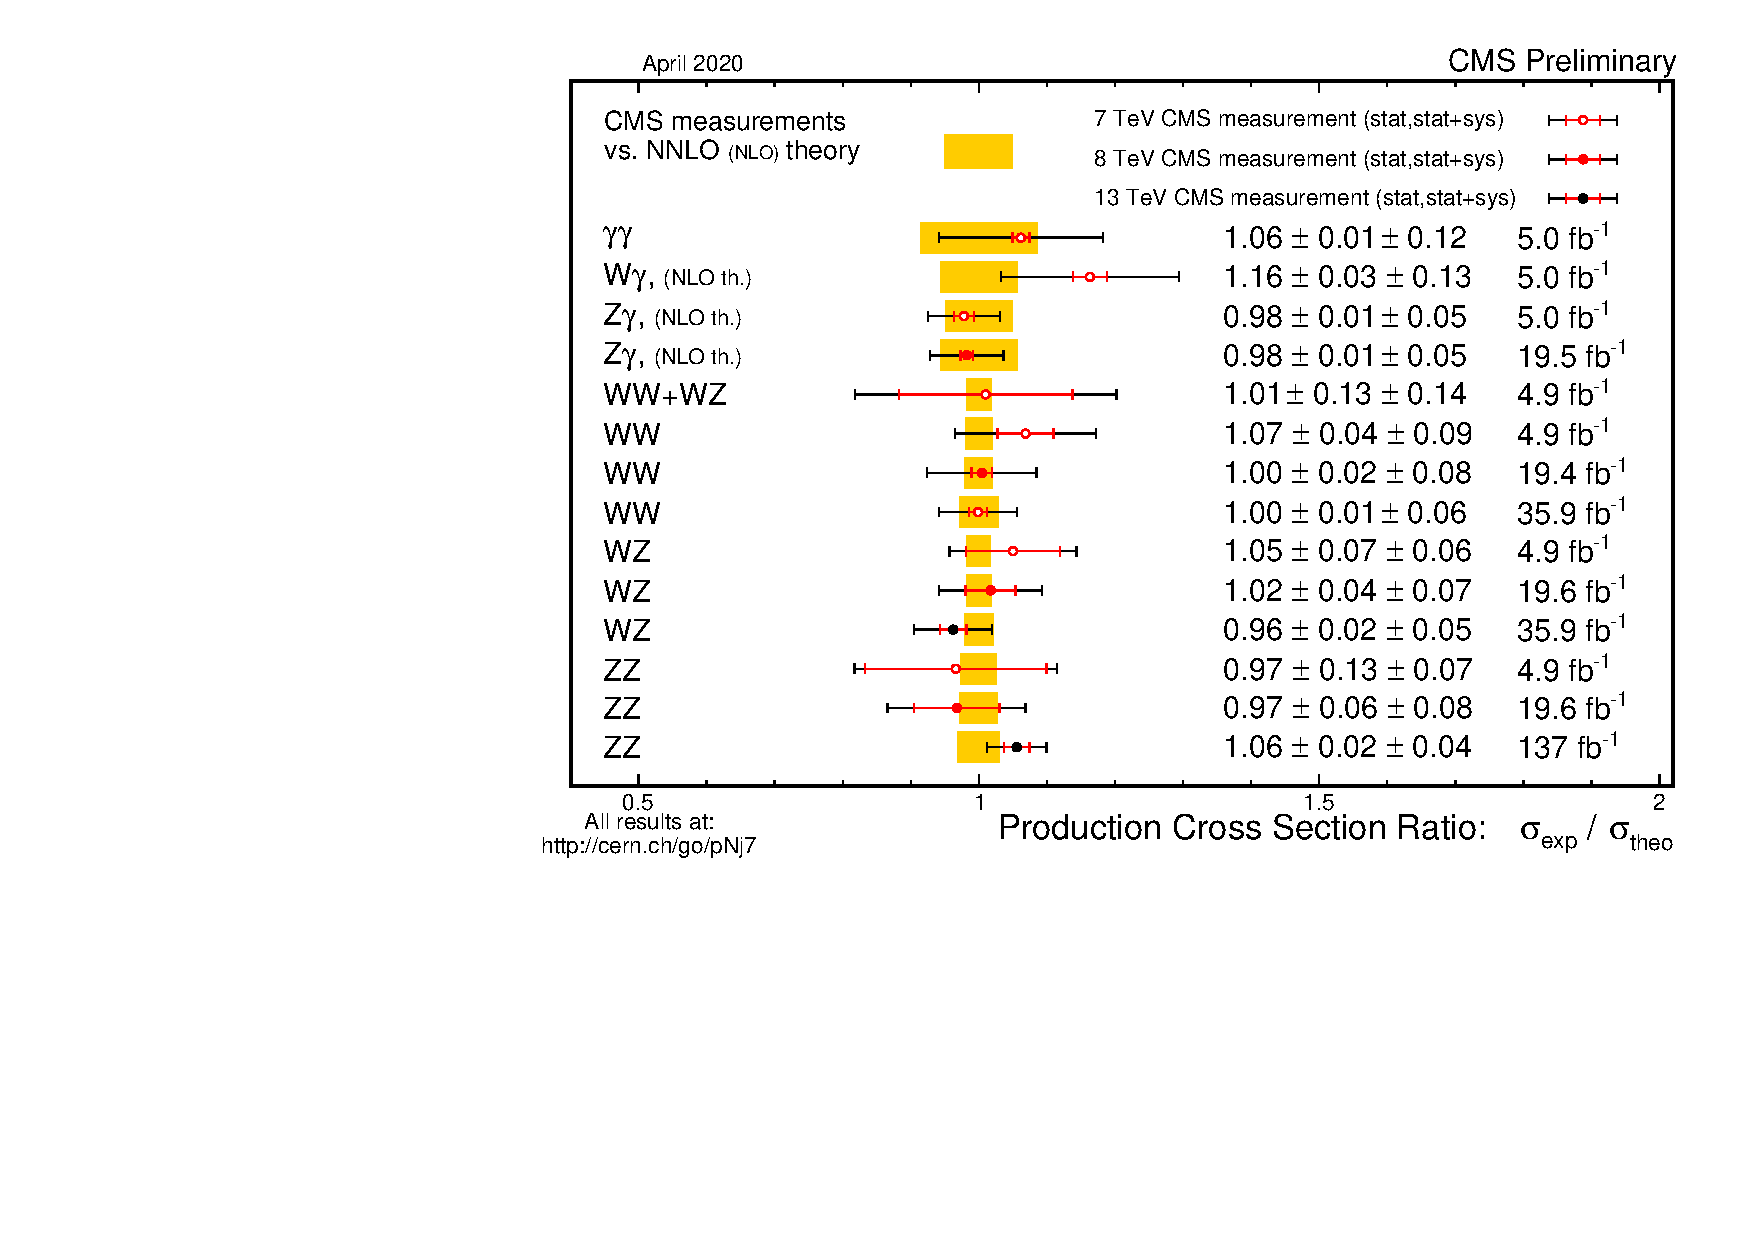
\includegraphics[width=\textwidth]{figures_and_tables/theory/sm_vbf_results.pdf}
    \caption{}
    \label{sm_vbf_results}
  \end{subfigure}
  \hfill
  \begin{subfigure}[htbp]{0.48\textwidth}
    \centering
    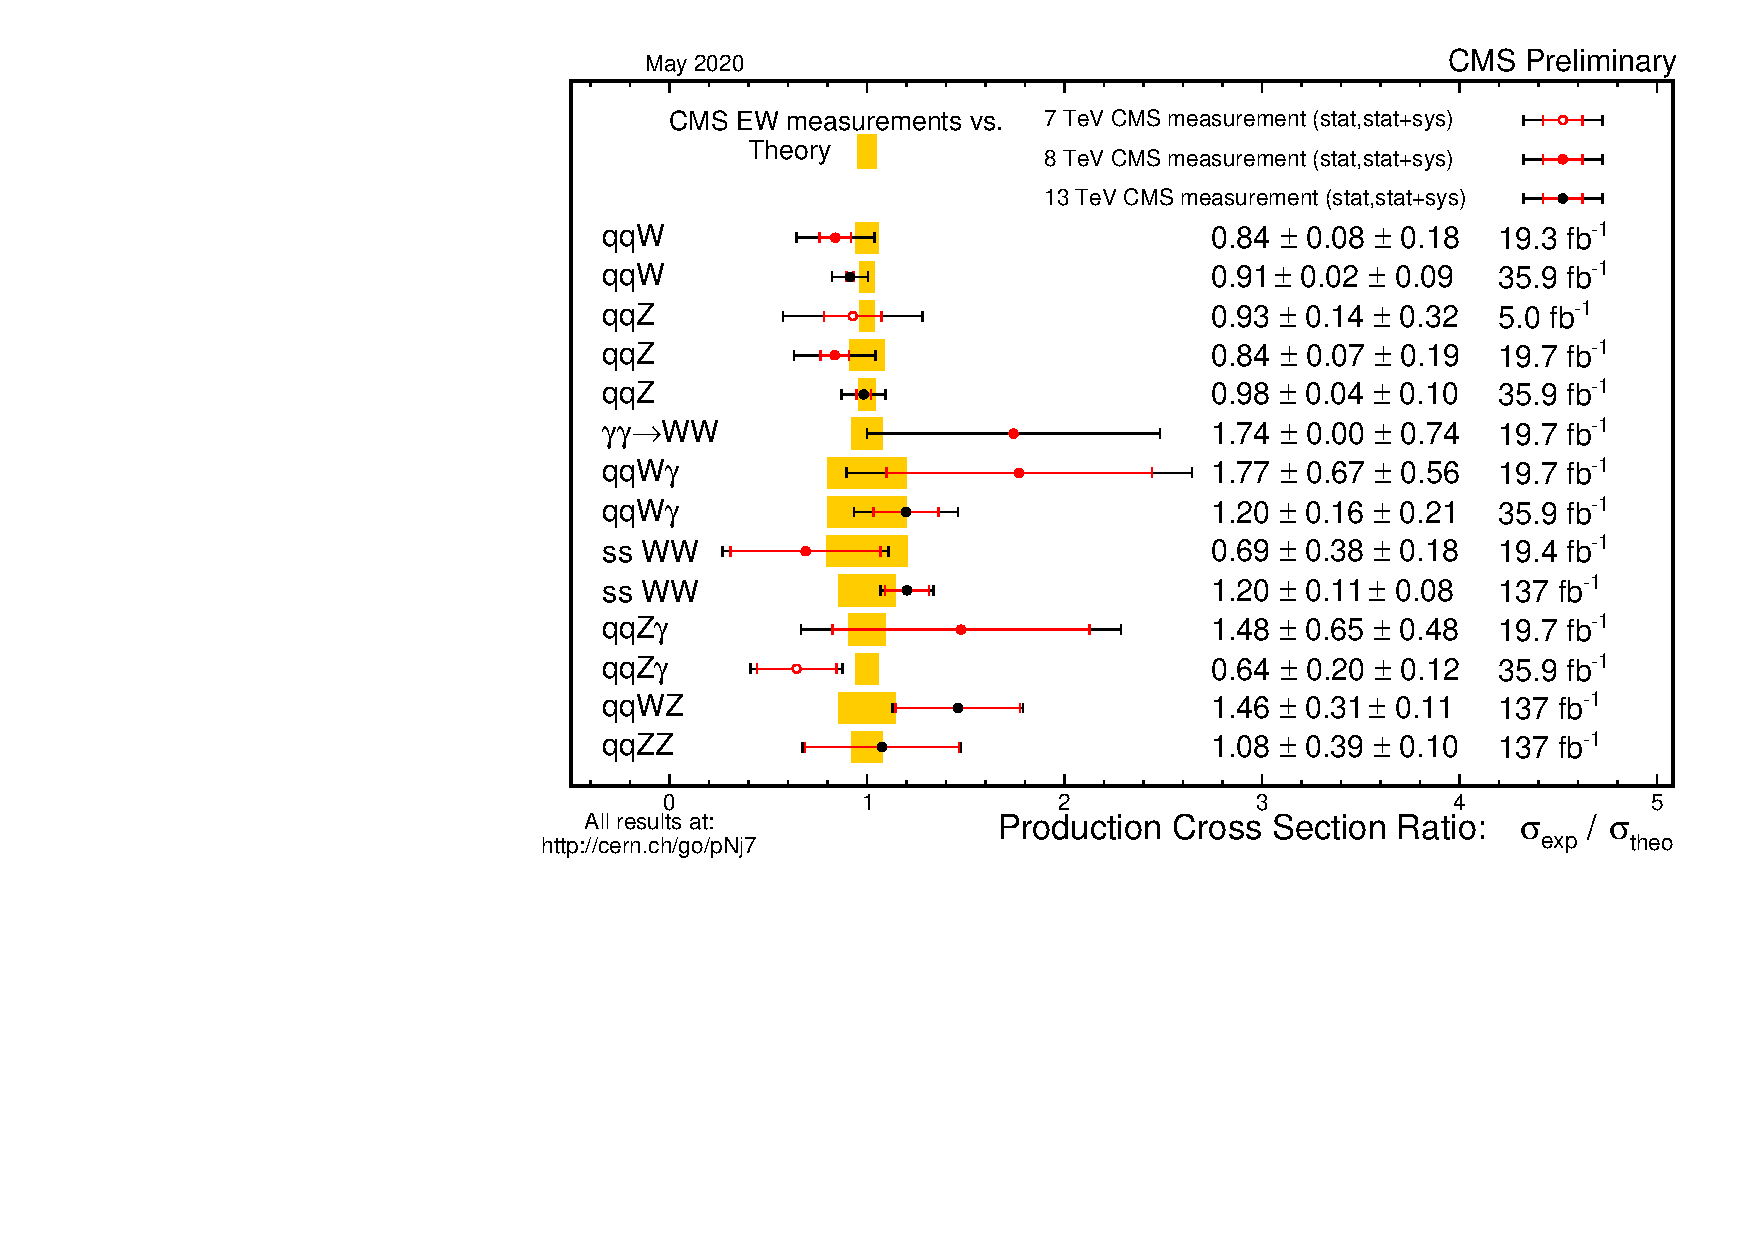
\includegraphics[width=\textwidth]{figures_and_tables/theory/sm_ewk_results.pdf}
    \caption{}
    \label{sm_ewk_results}
  \end{subfigure}
  \caption{(a) Di-boson cross section ratio comparison to theory: Theory predictions updated to latest NNLO calculations where available compared to predictions in the CMS papers and preliminary physics analysis summaries. Source:~\cite{cms_sm_xsec_summary}. (b) Summary of the cross sections of pure Electroweak (EWK) interactions among the gauge bosons presented as a ratio compared to theory. Source:~\cite{cms_sm_xsec_summary}.}
\end{figure}

\begin{sidewaysfigure}[htbp]
  \centering
  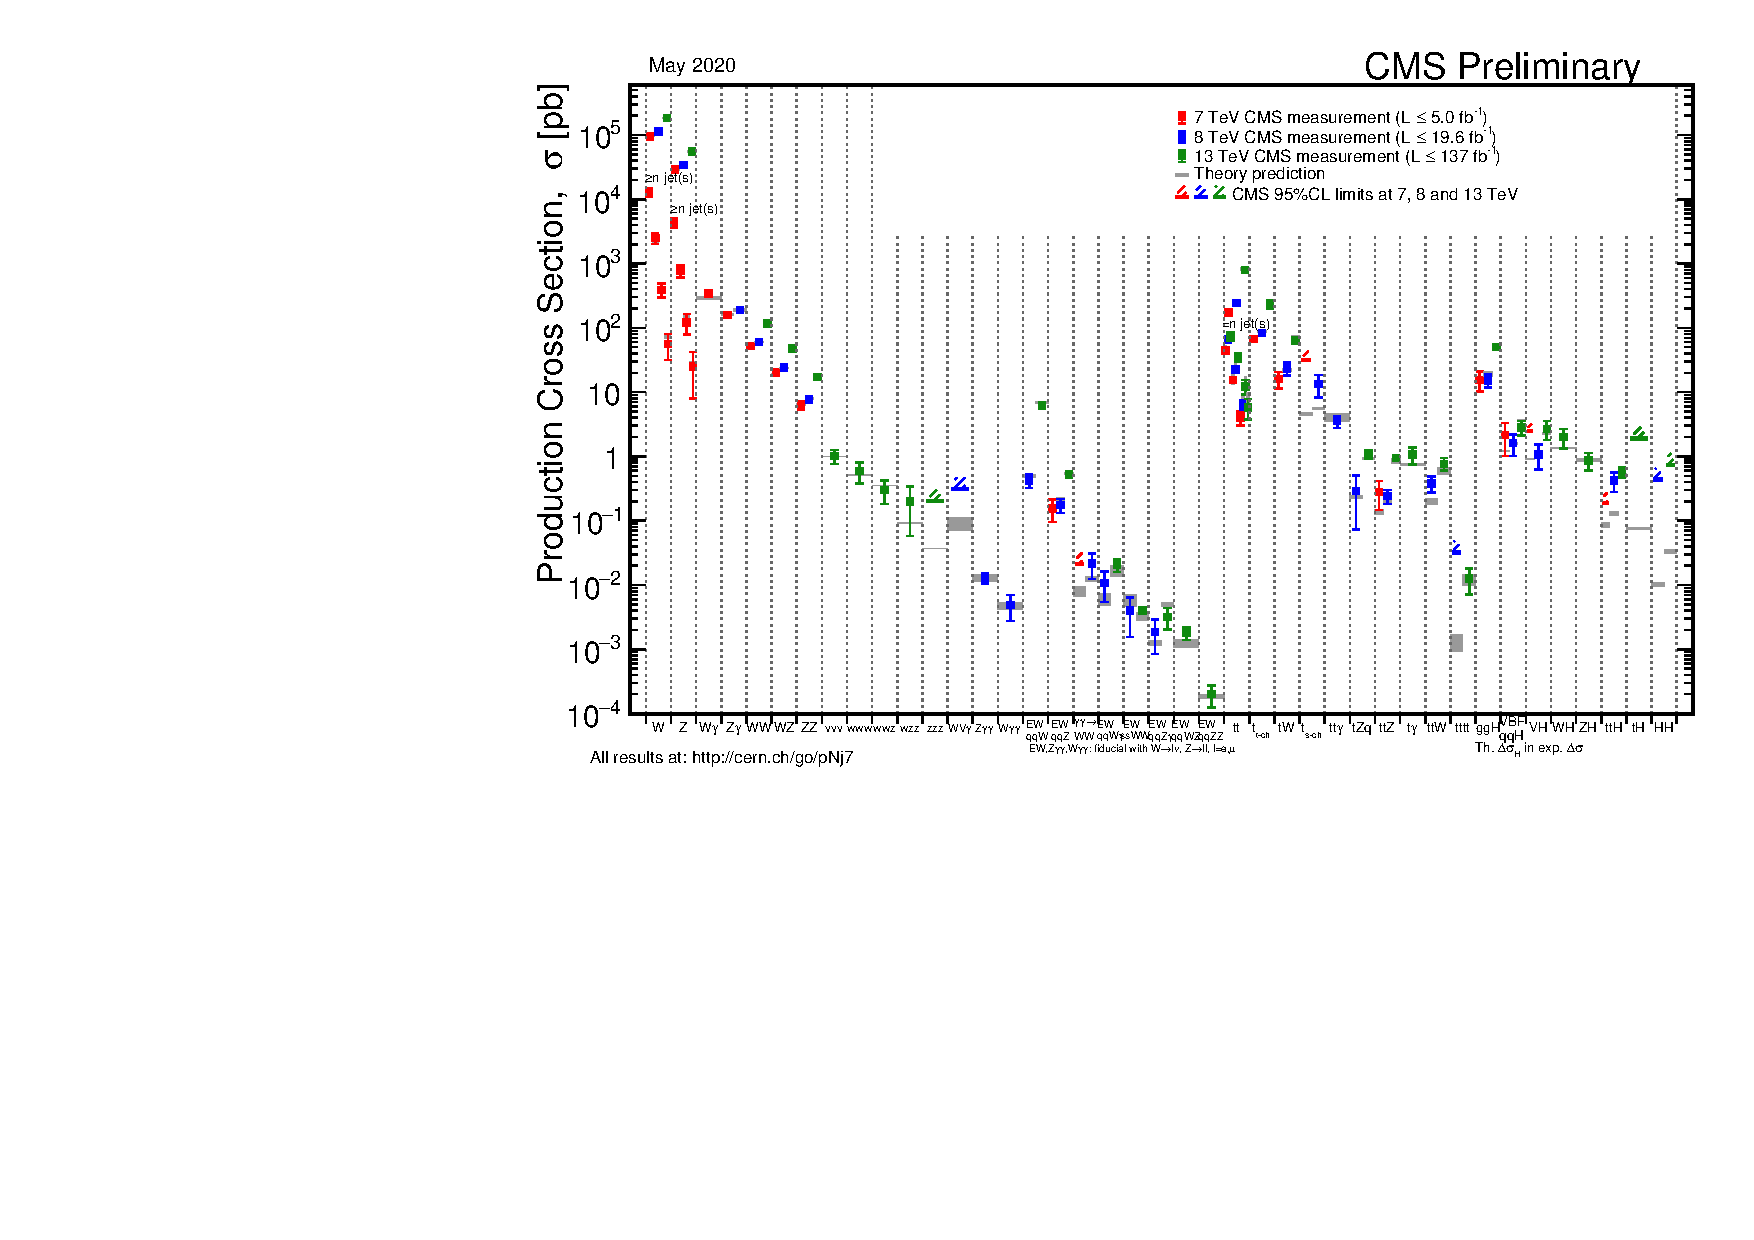
\includegraphics[width=\textwidth]{figures_and_tables/theory/cms_sm_xsec.pdf}
  \caption{Summary of the cross section measurements of Standard Model processes at CMS. Source:~\cite{cms_sm_xsec_summary}.}
  \label{cms_sm_xsec}
\end{sidewaysfigure}

The open questions above are not subjected to the SM scope, but even within the SM there still relevant precision measurements~\cite{sm_global_fit} that are important to understand the validity of the SM and what other questions lies about the SM, at the threshold of the LHC experiments precision.

\clearpage 